% Documentation example
% Author: Antoine de Barbarin
% Created at: April 5th, 2025
% Last modified at: April 5th, 2025

\documentclass{report}
\usepackage{amssymb}
\usepackage{thorgdocs}

% Set document variables
\renewcommand{\docname}{Home\&Co}
\renewcommand{\docsubtitle}{Ynov - Development Project}
\renewcommand{\authorname}{Antoine de Barbarin\\
                           Nicolas Moyon}
\renewcommand{\docdate}{April 5th, 2025}

% Link setup 
\linksetup

\begin{document}

\watermarklogo[\paperwidth/3,\paperheight/2-\textheight/6]{ui/assets/img/logo/logo.png}

% Title page
\coverpage

% Index and pagination
\indexpagination{ui/assets/img/logo/HomeNCo-logo.png}

\chapter{Presentation}\label{ch:presentation}

    This project is made by Computer Science students for an assignment involving a client application, in this case a website, and a real time interaction with the physical world via ESP32 boards.

    \textbf{Home\&Co} \emph{(Co for Connect, Control, Company)} is a project using \textbf{ESP32} microcontrollers and a \textbf{Raspberry Pi 3B+} to monitor, control and automate home appliances like the lights, heaters, front door, water valves for watering plants, etc.

    Its goals are to provide \textbf{security}, \textbf{control}, \textbf{comfort}, \textbf{peace of mind} and \textbf{energy saving} to your home.

    \section{Security}\label{sec:security}

        Our front door device will control the access policy of the front door of your home:
        \begin{itemize}
            \item \textbf{RFID} sensor needing a \textbf{badge} to open the door
            \item \textbf{doorbell button} ringing the bell and \textbf{notifying you on your phone}
            \item \textbf{locking mechanism} controlled \textbf{remotely} (no need to give keys to anybody)
            \item \textbf{presence detector} to \textbf{monitor} the activity in front of the door
            \item \textbf{house locking function} to \textbf{automatically turn off} all the lights and use all presence detectors as \textbf{intrusion detectors}
        \end{itemize}

    \section{Control}\label{sec:control}

        You can use the website to \textbf{remotely control at any time} the \emph{lights}, the \emph{door}, the \emph{heaters} and the \emph{watering of plants}.

        You have \textbf{full control of your house} from any device.

    \section{Comfort}\label{sec:comfort}

        You can \textbf{automate the heaters} to activate at any time of the day, to find a warm house when coming back from a hike, vacation or any activity.

    \section{Peace of mind}\label{sec:peace-of-mind}

        You will not have to go through your checklist three times or ask your neighbor to water your plants before going out!

        You can \textbf{monitor your house from any device} using the website in \textbf{real time}: from the \emph{presence detectors} to the \emph{lights}, \emph{heaters}, \emph{humidity of the plants} and \emph{temperature of any room}.

    \section{Energy saving}\label{sec:energy-saving}

        No need to keep heating your home when you're not there!

        You will be able to control and monitor the \textbf{heaters} remotely and according to your needs and presence at home.

        You will also be able to \textbf{monitor the energy of specific high consumption appliances} with our \textbf{smart power outlet} and control them remotely, and even give them schedules to be working or not.

\chapter{System Design}\label{ch:system-design}

    \section{Needs Analysis}\label{sec:needs-analysis}

        \begin{itemize}
        \item \textbf{Goal}: fully functional home with remote control (from the web browser)
        \item \textbf{Security Constraint}: no direct access to ESP32 microcontrollers with their sensors and actuators, to database, MQTT or backend application.
        \item \textbf{Components}:
            \begin{itemize}
                \item Raspberry Pi 3 or more for Wi-Fi access point, MQTT, backend app and webserver.
                \item ESP32 for sensors \& actuators
            \end{itemize}
        \end{itemize}

    \section{Technical choices}\label{sec:technical-choices}

        \begin{itemize}
            \item \textbf{Golang} for the backend app and webserver with GORM:
                \begin{itemize}
                \item Golang is an excellent choice for building efficient, concurrent applications due to its simplicity and strong type system.
                \item The Go standard library is comprehensive, making it easy to handle tasks like networking, file I/O, and concurrency.
                \item GORM, a popular ORM for Golang, simplifies database interactions by providing a clean and intuitive API.
                \end{itemize}

            \item \textbf{PostgreSQL} for the database:
                \begin{itemize}
                \item PostgreSQL is an advanced, open source relational database management system known for its robustness, scalability, and ACID compliance.
                \item It offers features like transactions, indexing, and support for complex data types, making it ideal for handling diverse and large-scale applications.
                \end{itemize}

            \item \textbf{Mosquitto} for the MQTT broker:
                \begin{itemize}
                \item Mosquitto is a lightweight, open source MQTT broker that's highly reliable and easy to configure.
                \item Its simplicity and performance make it an excellent choice for real-time communication between devices and services, especially in scenarios where low latency and high availability are crucial.
                \end{itemize}

            \item \textbf{RaspAP} for the Wi-Fi Access Point in the Raspberry Pi:
                \begin{itemize}
                \item RaspAP provides a user-friendly interface for setting up and managing a Wi-Fi access point on a Raspberry Pi.
                \item It simplifies the process of configuring network settings, security protocols, and other related tasks, making it accessible even to users with limited technical expertise.
                \end{itemize}

            \item \textbf{Websocket} between JavaScript clients and Golang server:
                \begin{itemize}
                \item Websockets provide full-duplex communication channels over a single TCP connection, enabling real-time data exchange between the frontend and backend.
                \item This is particularly useful for applications requiring immediate updates and interactions, such as chat applications or live dashboards.
                \end{itemize}

            \item \textbf{PlatformIO} and \textbf{C}/\textbf{C++} for the ESP32:
                \begin{itemize}
                \item PlatformIO offers a unified development environment for embedded systems, making it easy to manage multiple projects and boards.
                \item It supports a wide range of platforms and tools, including C/C++, which is ideal for writing efficient and low-level code for microcontrollers like the ESP32.
                \end{itemize}
        \end{itemize}

    \section{Basic features}\label{sec:basic-features}

        \begin{itemize}
            \item Monitoring sensors with the web interface
            \item Controlling actuators from the web interface
            \item Data collection in the database
            \item Light and temperature management
            \item Front door monitoring with \inlinecode{RFID} badge
        \end{itemize}

    \section{Additional features (future release)}\label{sec:additional-features-(future-release)}

        \begin{itemize}
            \item Energy consumption management
            \item Shutter and window management
            \item Fire and smoke detection
            \item Alarm mode
            \item Ventilation management
            \item Scheduler for actuators (heaters, light, shutters, ventilation)
            \item Statistics and prevision dashboards
        \end{itemize}

    \section{Components Architecture}\label{sec:components-architecture}

        \subsection{Overall Infrastructure}\label{subsec:overall-infrastructure}

        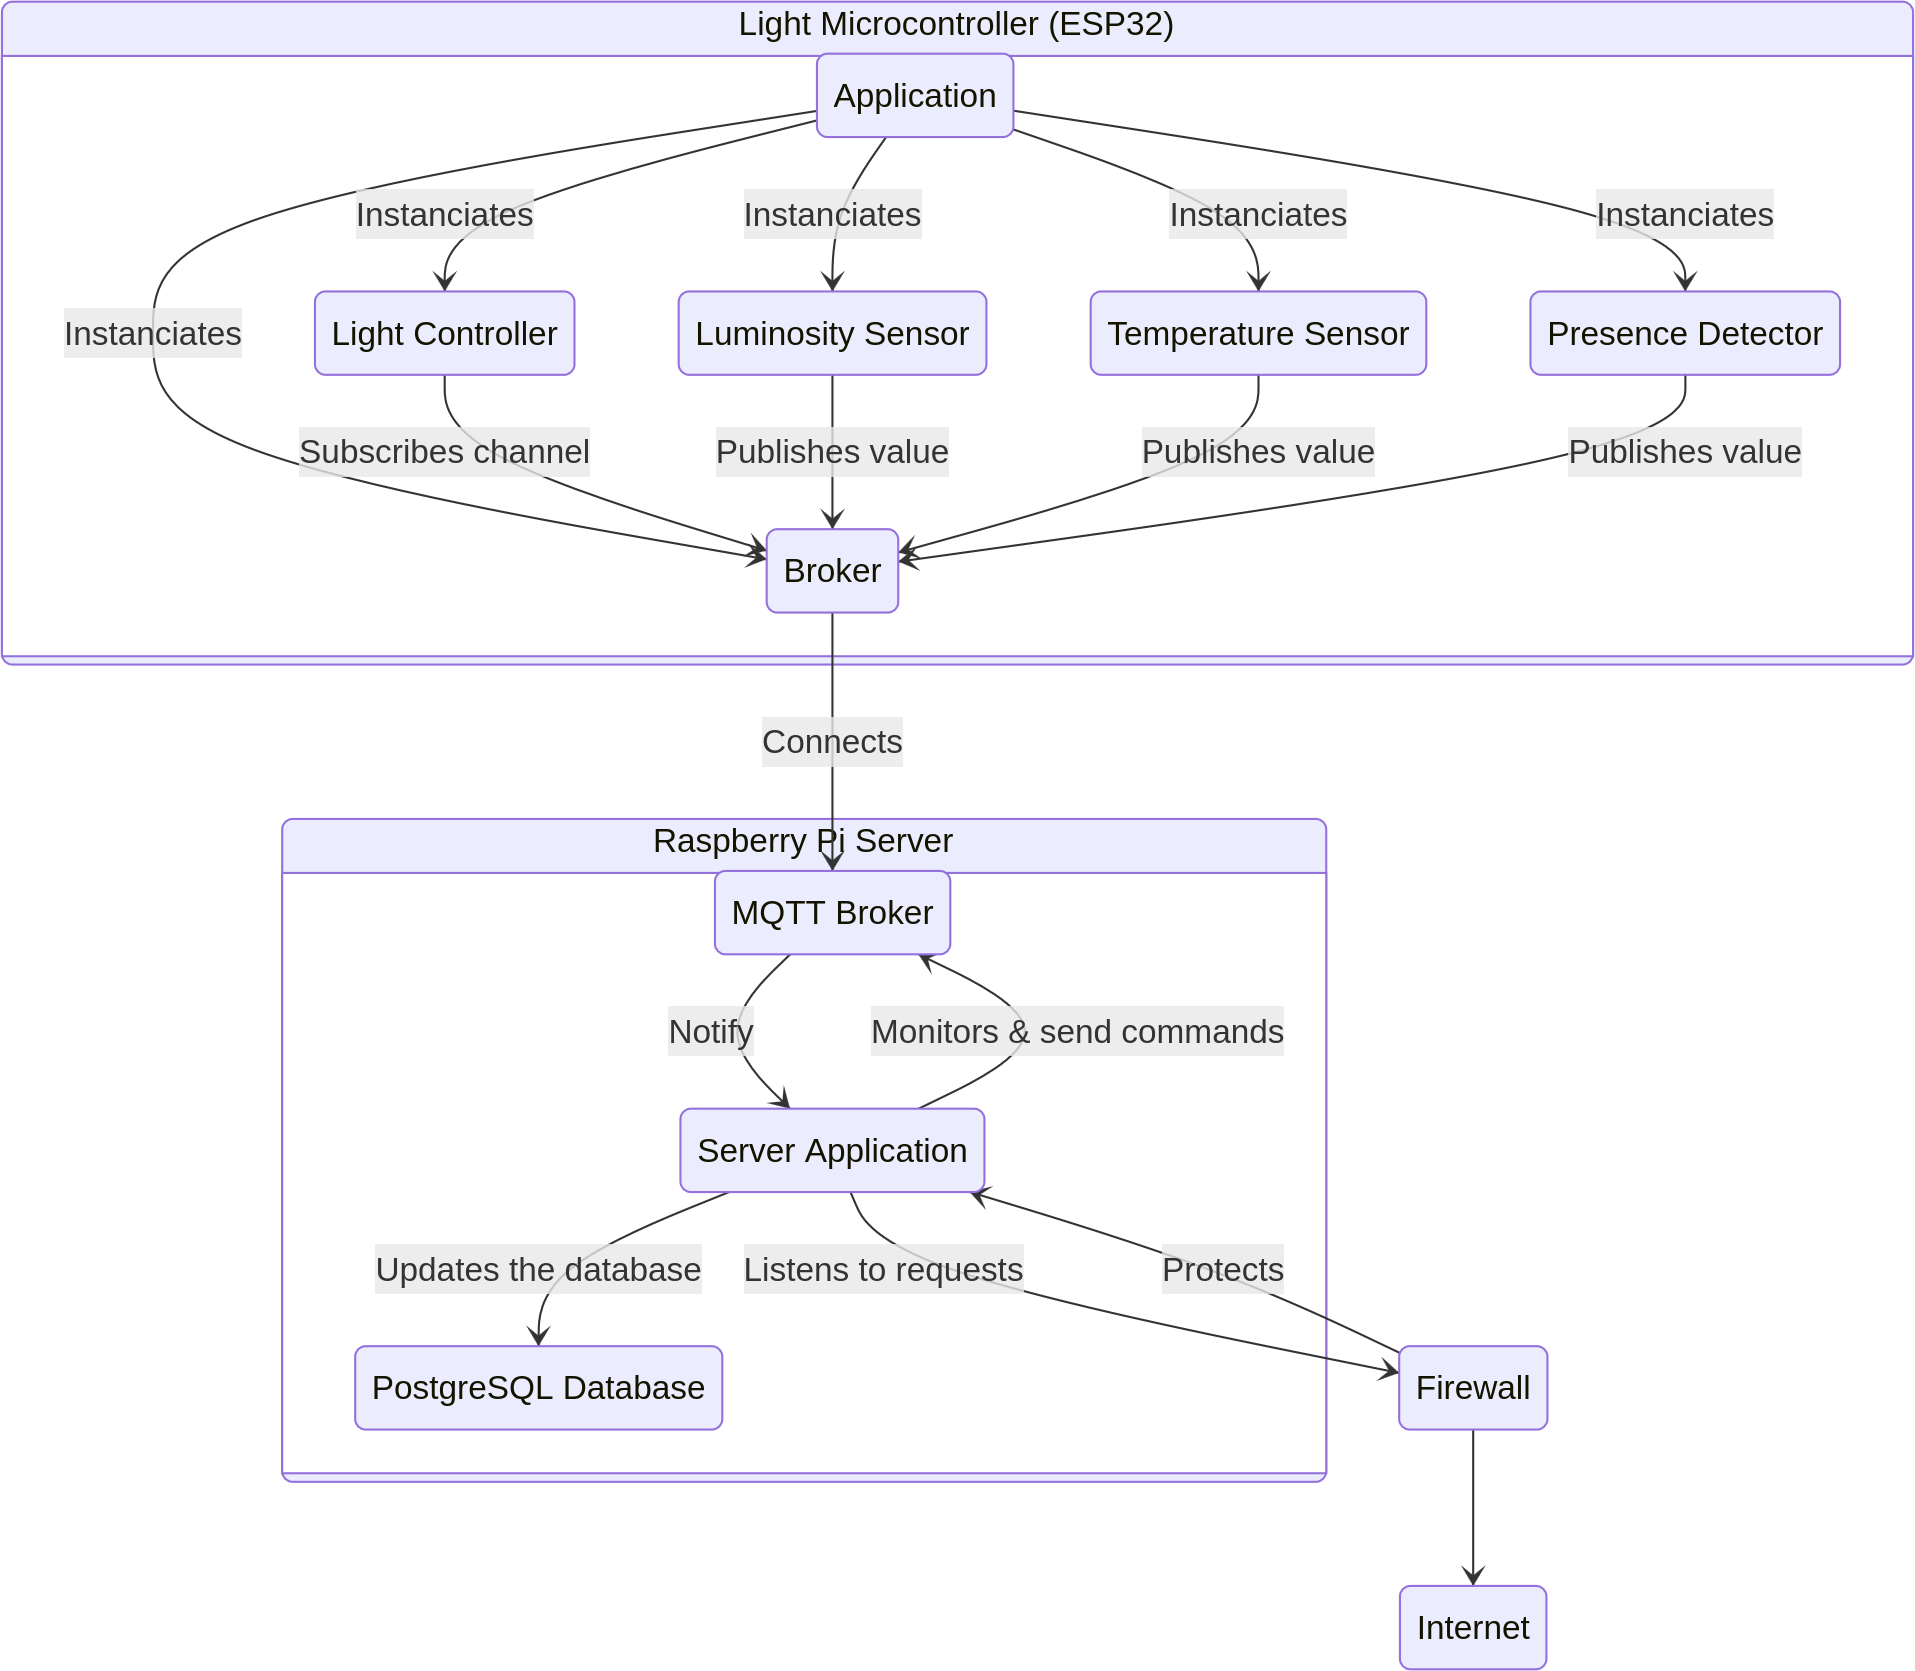
\includegraphics[width=17cm]{ui/assets/img/overall-infrastructure}

        \subsection{Database}\label{subsec:database}

            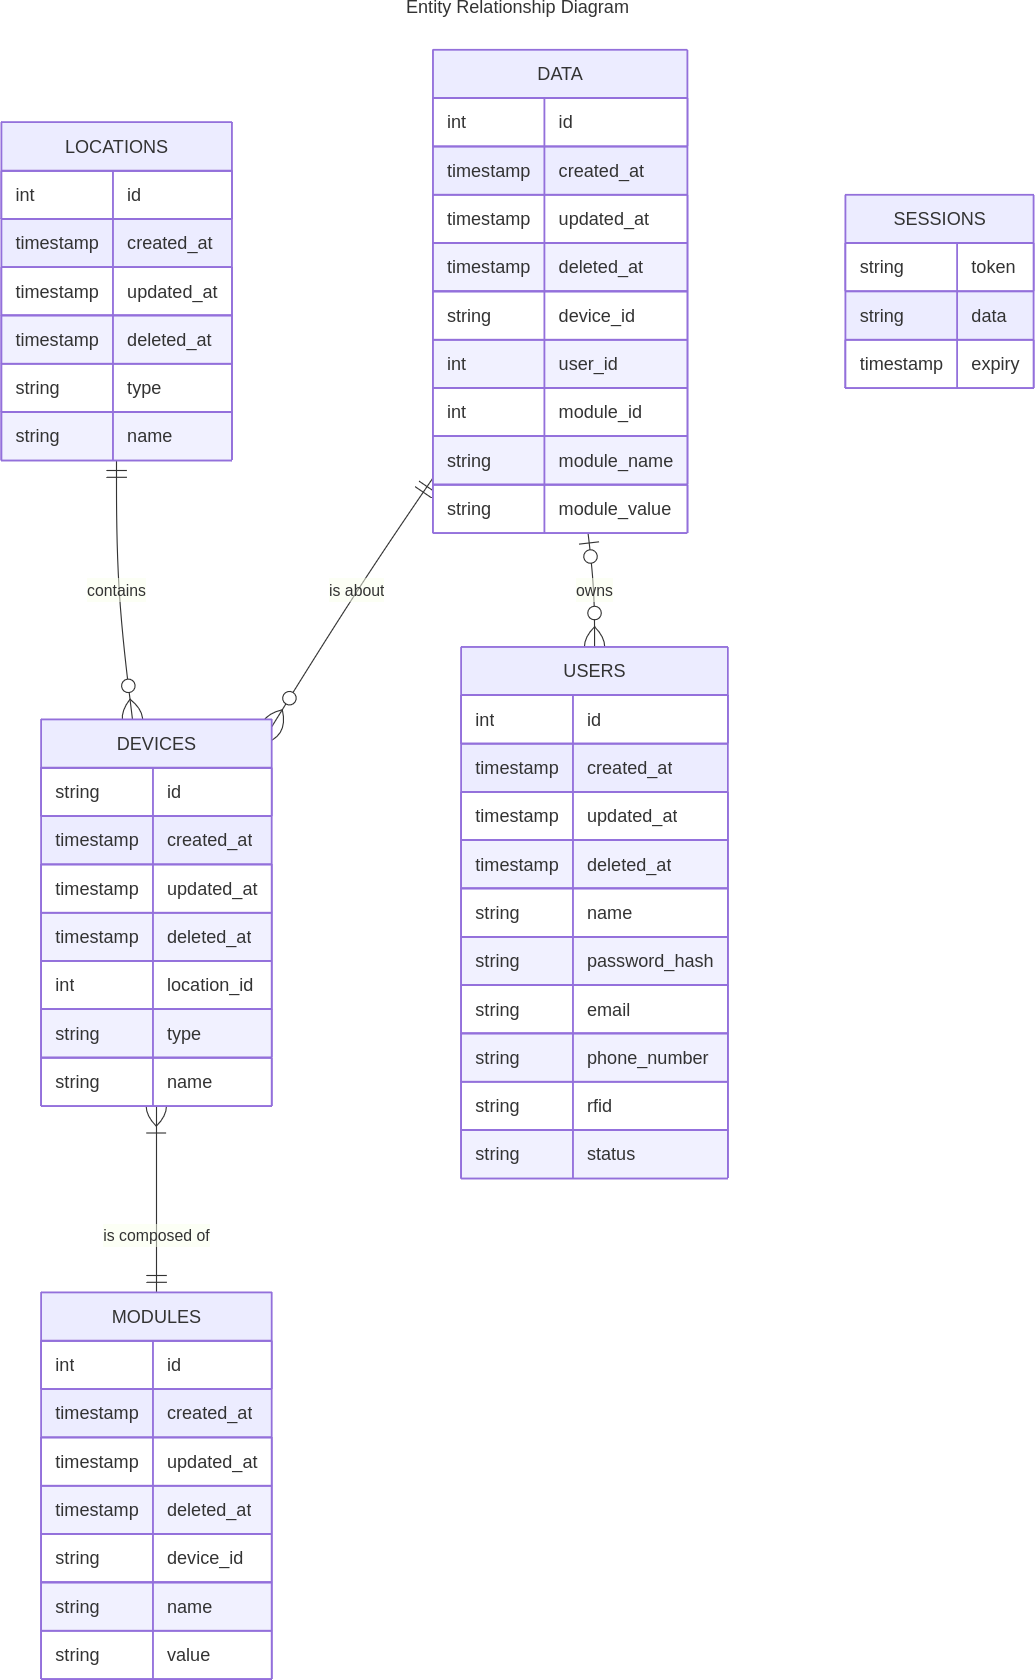
\includegraphics[height=22cm]{ui/assets/img/database}

        \subsection{MQTT}\label{subsec:mqtt}

            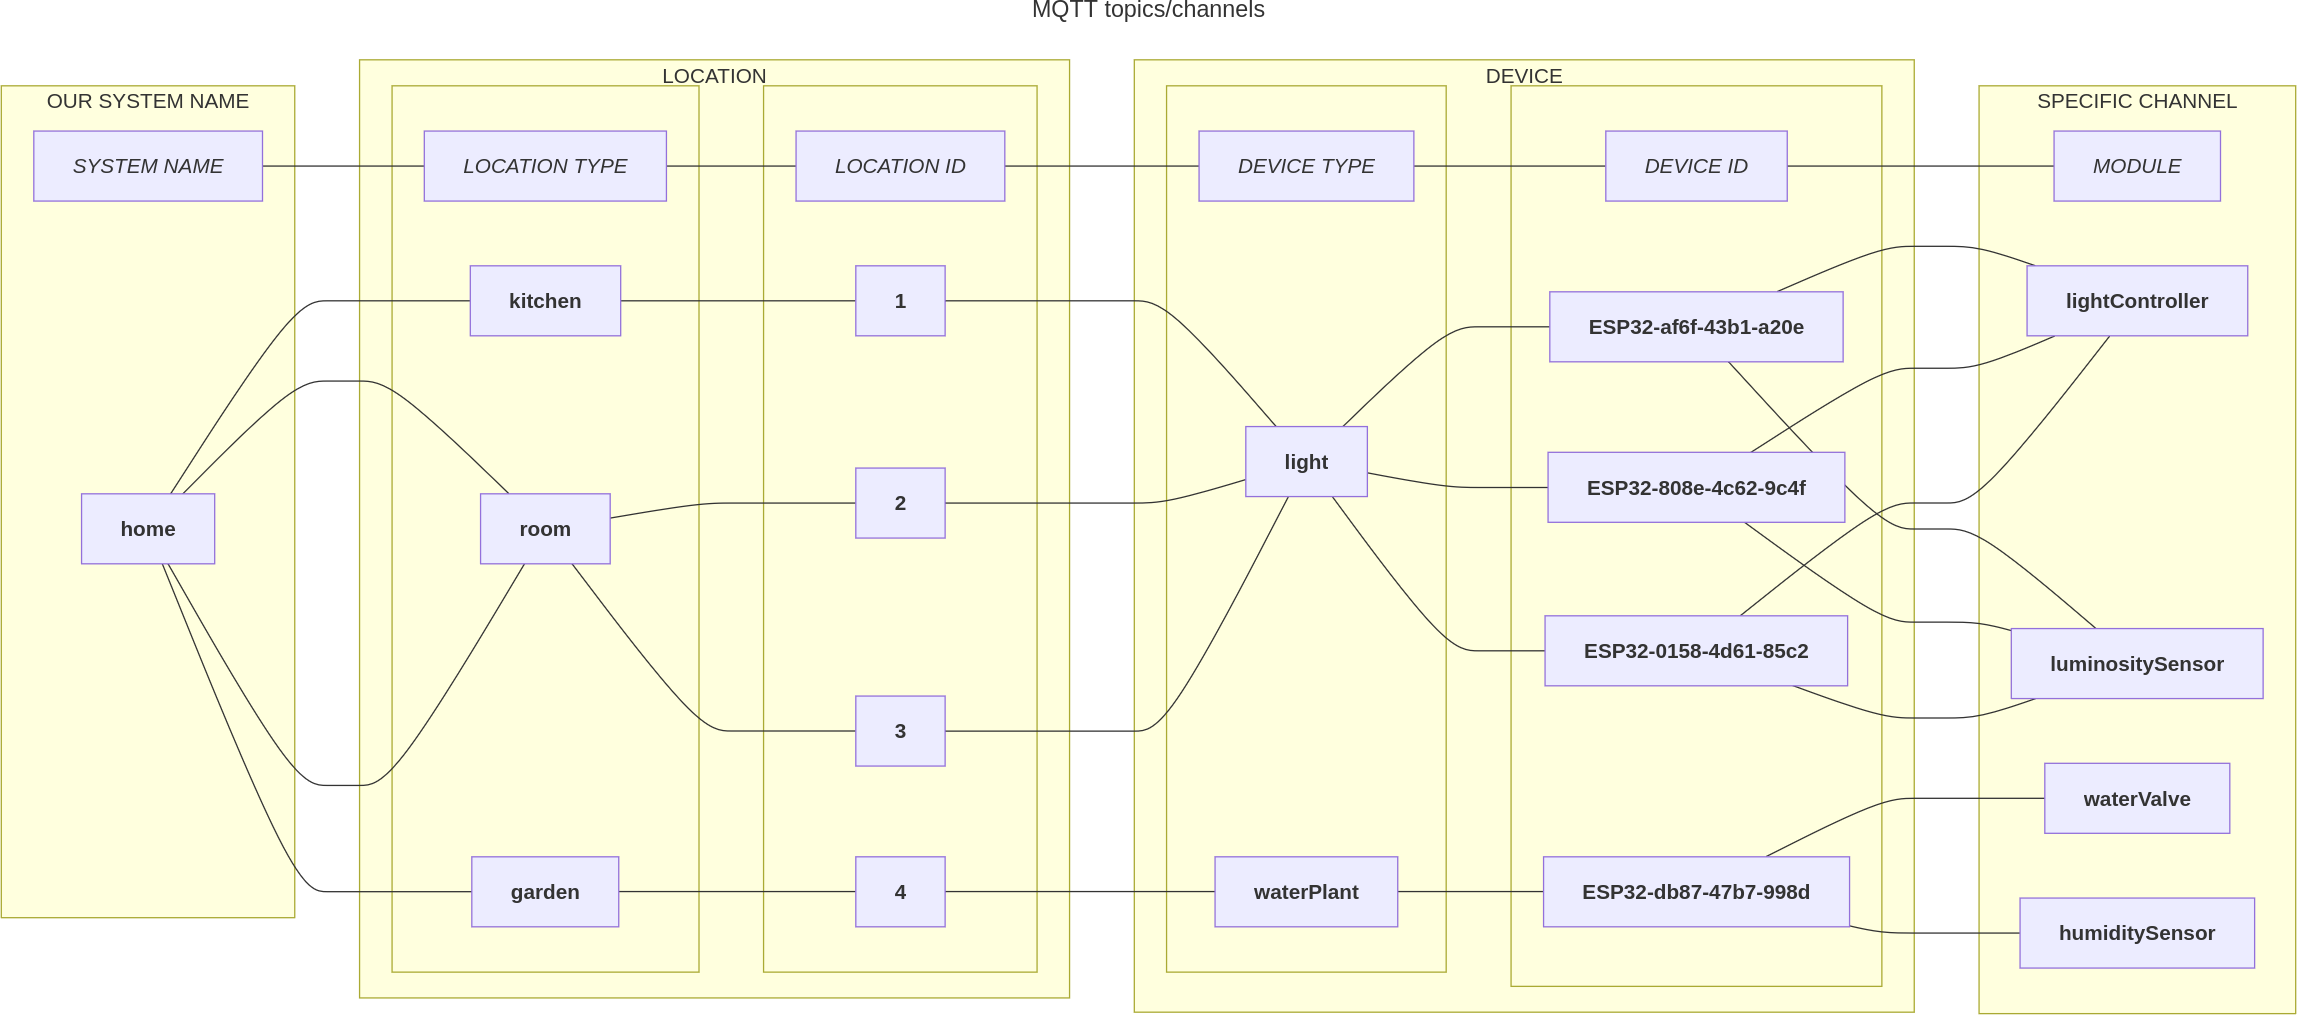
\includegraphics[width=17cm]{ui/assets/img/mqtt-topics}

        \subsection{Webserver File Architecture}\label{subsec:webserver-file-architecture}

            \begin{termbox}
            |-- cmd
            |   |-- web
            |       |-- context.go
            |       |-- handlers.go
            |       |-- helpers.go
            |       |-- main.go
            |       |-- middleware.go
            |       |-- models.go
            |       |-- routes.go
            |       |-- server.go
            |       |-- templates.go
            |-- go.mod
            |-- go.sum
            |-- internal
            |   |-- data
            |   |   |-- broker.go
            |   |   |-- consumption-sensor.go
            |   |   |-- data.go
            |   |   |-- device.go
            |   |   |-- imodule.go
            |   |   |-- light-controller.go
            |   |   |-- light-sensor.go
            |   |   |-- location.go
            |   |   |-- luminosity-sensor.go
            |   |   |-- models.go
            |   |   |-- module.go
            |   |   |-- presence-detector.go
            |   |   |-- reset.go
            |   |   |-- startup.go
            |   |   |-- subscription.go
            |   |   |-- temperature-sensor.go
            |   |   |-- value-conversion.go
            |   |-- mailer
            |   |   |-- mailer.go
            |   |   |-- templates
            |   |       |-- alert-notification.tmpl
            |   |-- validator
            |       |-- validator.go
            |-- README.md
            |-- ui
            |   |-- assets
            |   |   |-- css
            |   |   |   |-- base.scss
            |   |   |   |-- style.scss
            |   |   |-- font
            |   |   |   |-- Dosis-VariableFont_wght.ttf
            |   |   |-- img
            |   |       |-- logo
            |   |           |-- logo.png
            |   |-- efs.go
            |   |-- templates
            |       |-- base.tmpl
            |       |-- pages
            |       |   |-- error.tmpl
            |       |   |-- home.tmpl
            |       |-- partials
            |-- vendor
            \end{termbox}

        \subsection{ESP32 C++ File Architecture}\label{subsec:esp32-c++-file-architecture}

            \begin{termbox}
            |-- include
            |   |-- Application.h
            |   |-- Broker.h
            |   |-- ConsumptionSensor.h
            |   |-- environment.h
            |   |-- IModule.h
            |   |-- IObservable.h
            |   |-- IObserver.h
            |   |-- LightController.h
            |   |-- LightSensor.h
            |   |-- LuminositySensor.h
            |   |-- ModuleFactory.h
            |   |-- MyAny.h
            |   |-- PresenceDetector.h
            |   |-- README
            |   |-- TemperatureSensor.h
            |   |-- utils.h
            |-- lib
            |   |-- README
            |   |-- xht11
            |       |-- xht11.cpp
            |       |-- xht11.h
            |-- LICENSE
            |-- platformio.ini
            |-- README.md
            |-- src
               |-- Application.cpp
               |-- Broker.cpp
               |-- ConsumptionSensor.cpp
               |-- HomeIoT.ino
               |-- LightController.cpp
               |-- LightSensor.cpp
               |-- LuminositySensor.cpp
               |-- ModuleFactory.cpp
               |-- PresenceDetector.cpp
               |-- TemperatureSensor.cpp
               |-- utils.cpp
            \end{termbox}

        \subsection{ESP32 Class Diagram}\label{subsec:esp32-class-diagram}

            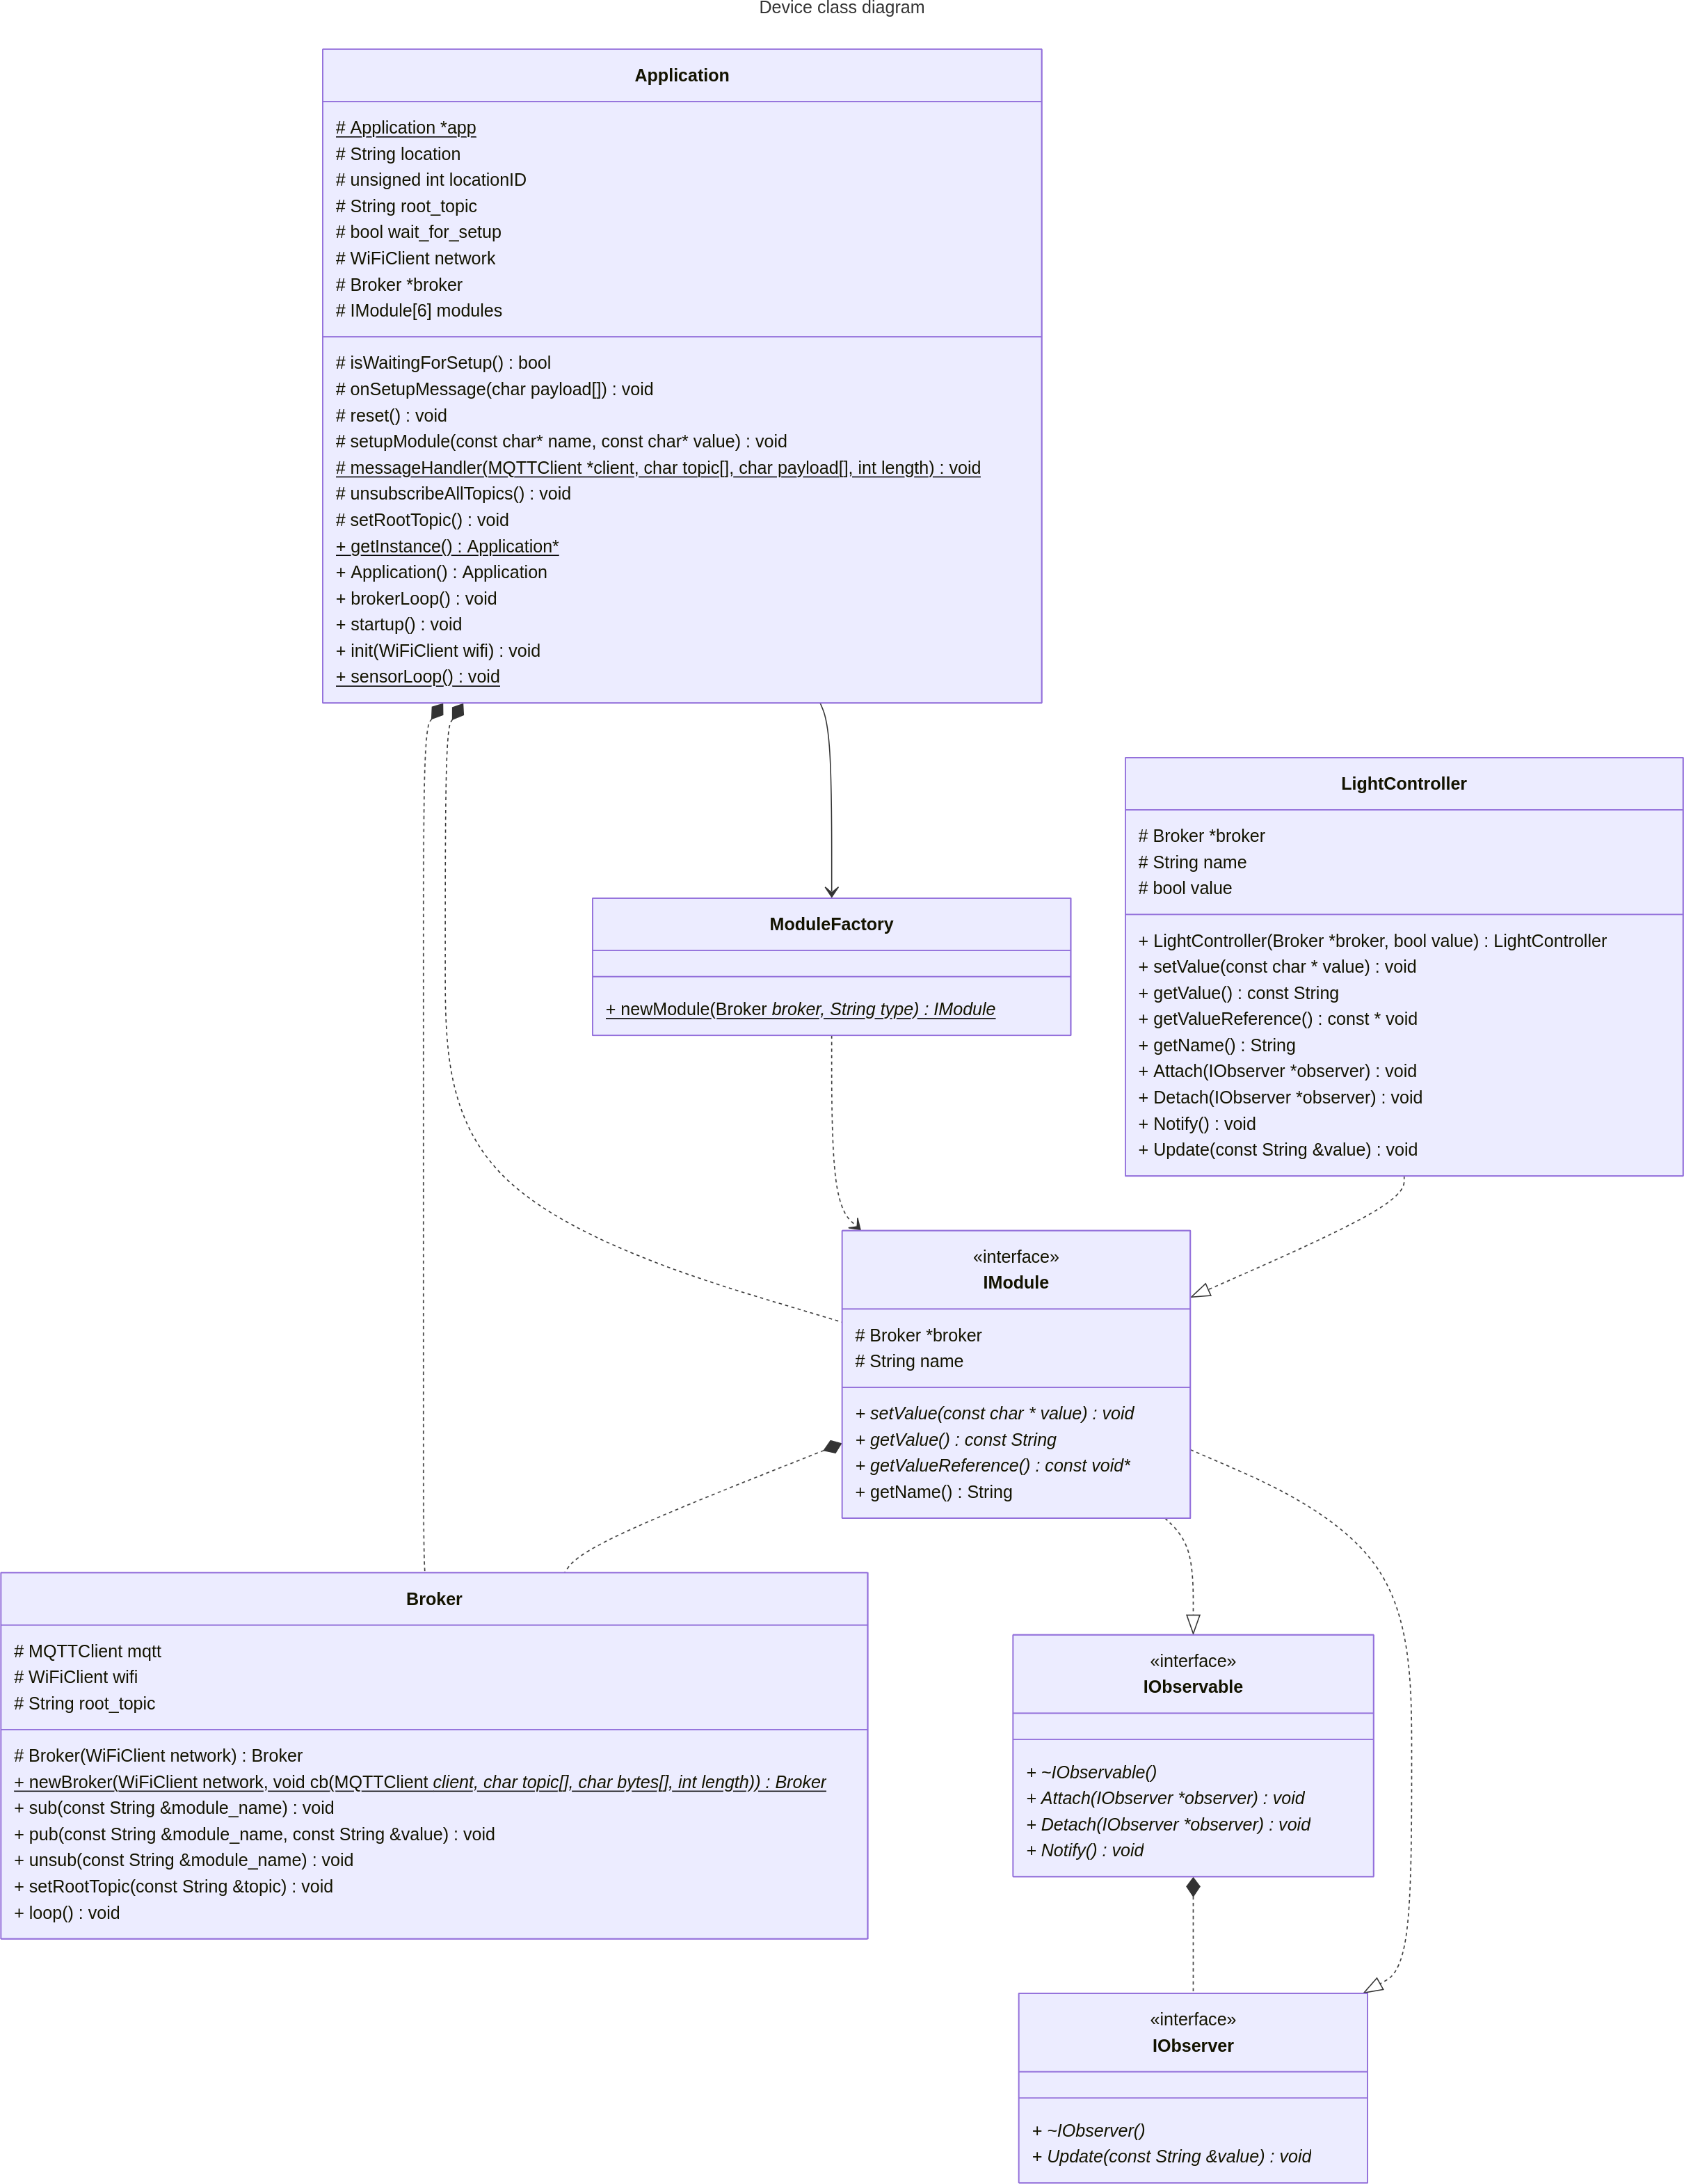
\includegraphics[width=17cm]{ui/assets/img/esp32-class-diagram}

        \subsection{Setup/Startup}\label{subsec:setup/startup}

            \begin{termbox}
            {
                "id": "ESP32-af6f-43b1-a20e",
                "type": "light",
                "location_id": 3,
                "location_type": "room",
                "location_name": "room 3",
                "modules": [
                    {
                        "name": "lightController",
                        "value": "False"
                    },
                    {
                        "name": "lightSensor",
                        "value": "True"
                    },
                    {
                        "name": "luminositySensor",
                        "value": "150.0"
                    },
                    {
                        "name": "presenceDetector",
                        "value": "True"
                    },
                    {
                        "name": "temperatureSensor",
                        "value": "22.5"
                    },
                    {
                        "name": "consumptionSensor",
                        "value": "32.45"
                    }
                ]
            }
            \end{termbox}

        \subsection{Setup Sequence Diagram}\label{subsec:setup-sequence-diagram}

            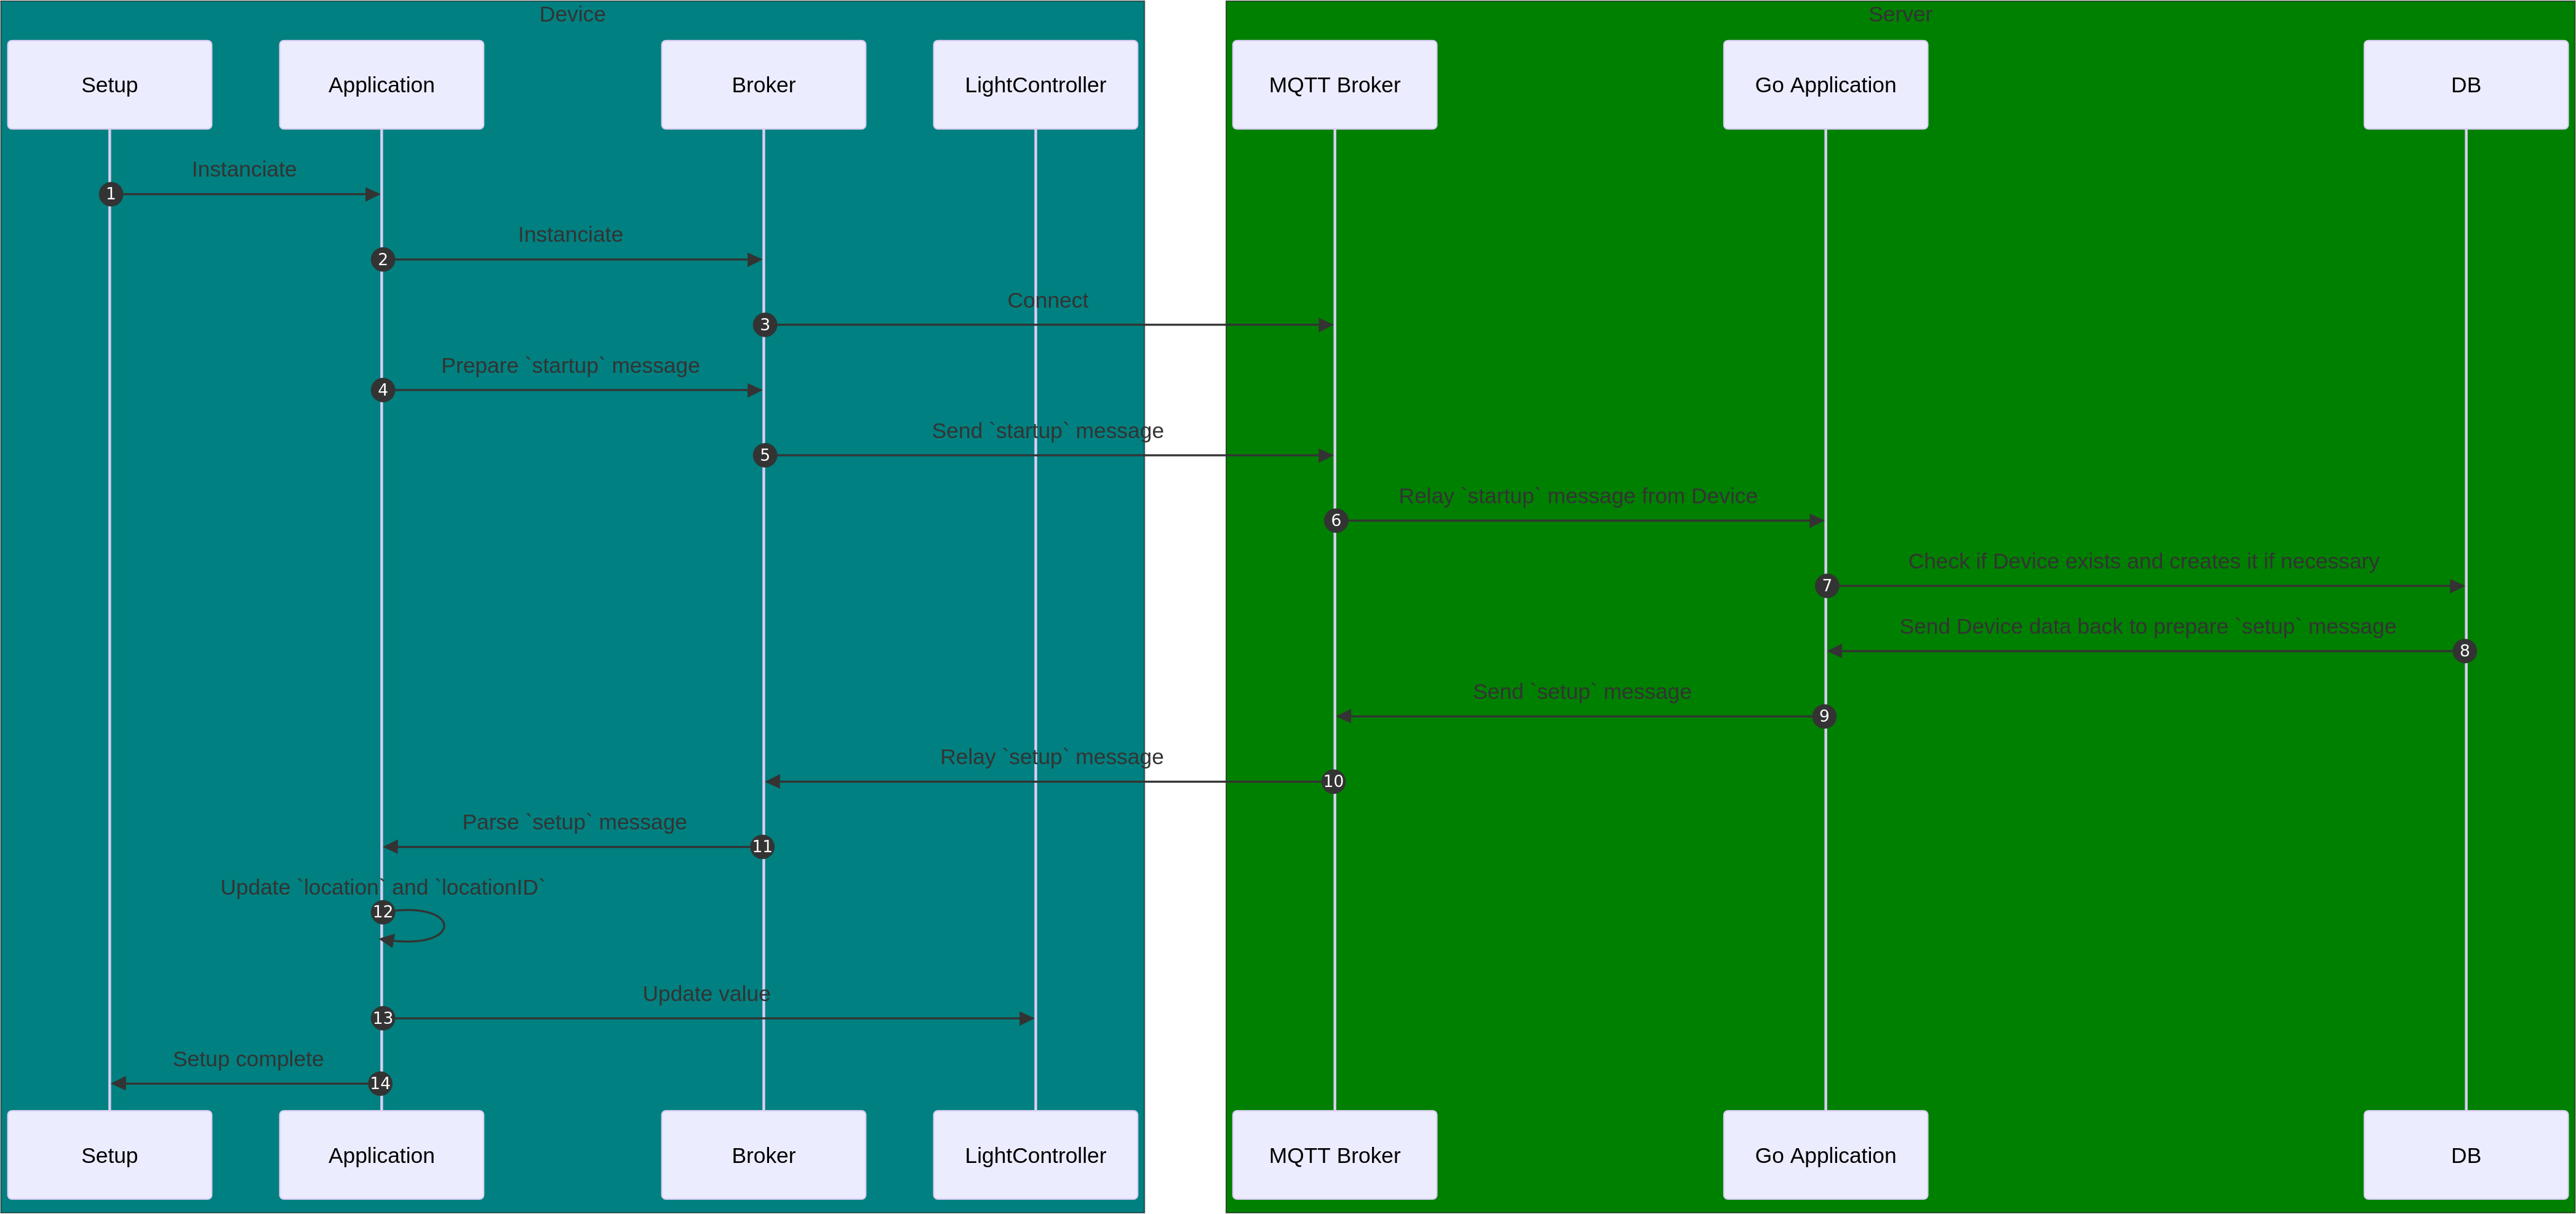
\includegraphics[width=17cm]{ui/assets/img/setup-sequence-diagram}

\chapter{Project Management}\label{ch:project-management}

    \section{Role Management}\label{sec:role-management}

        \begin{itemize}
            \item \textbf{Overall structure}: Antoine \& Nicolas
            \item \textbf{Documentation}: Antoine \& Nicolas
            \item \textbf{MQTT topics}: Antoine
            \item \textbf{Raspberry Pi setup}: Antoine
            \item \textbf{ESP32 structure \& code}: Antoine \& Nicolas
            \item \textbf{Database}: Antoine \& Nicolas
            \item \textbf{Golang webserver \& Application}: Antoine \& Nicolas
            \item \textbf{Frontend}: Antoine
            \item \textbf{Websockets}: Nicolas
        \end{itemize}

    \section{Workflow}\label{sec:workflow}

        We organized our project and advancement using an agile workflow with sprints.

        \subsection{Sprints}\label{subsec:sprints}

            \begin{itemize}
                \item[$\boxtimes$] \textbf{Project Structure}: 07/03 - 14/03
                \item[$\boxtimes$] \textbf{MQTT topics}: 07/03 - 14/03
                \item[$\boxtimes$] \textbf{Database}: 10/03 - 14/03
                \item[$\boxtimes$] \textbf{ESP32 Structure}: 14/03 - 21/03
                \item[$\boxtimes$] \textbf{Raspberry Pi Setup}: 14/03 - 24/03
                \item[$\boxtimes$] \textbf{ESP32 Code}: 14/03 - 24/03
                \item[$\square$] \textbf{Golang Webserver \& Application}: 10/03 - ongoing
                \item[$\square$] \textbf{Websockets}: 07/04 - ongoing
                \item[$\square$] \textbf{Frontend}
            \end{itemize}

    \section{Issues}\label{sec:issues}

        \begin{itemize}
            \item \textbf{System design}: implementing logic and standards with specific constraints.\\
                We resolved this issue making schemas and lists of constraints on paper to have a better overview and be able to think more properly.
            \item \textbf{Environment differences} between Linux \& Windows (terminal commands, environment variables).\\
                This issue was resolved creating a \emph{powershell} script that loads in the current terminal session all \emph{environment variables} for Windows.
        \end{itemize}

\end{document}

